\documentclass[a4paper]{article}
\usepackage[14pt]{extsizes} 
\usepackage[utf8]{inputenc}
\usepackage[english, russian]{babel}
\usepackage{amsmath}
\usepackage{amsfonts}
\usepackage{amssymb}
\usepackage{graphicx}
\usepackage{indentfirst}
\usepackage{mathtools}
\begin{document}
\begin{center}
\hfill \break
{\large МИНЕСТЕРСТВО НАУКИ ВЫСШЕГО ОБРАЗОВАНИЯ РОССИЙСКОЙ ФЕДЕРАЦИИ}\\
{\large Федеральное государственное бюджетное образовательное учереждение высшего образования}\\
\hfill \break
{\large \textbf{"КУБАНСКИЙ ГОСУДАРСТВЕННЫЙ УНИВЕРСИТЕТ"}} \\
\hfill \break
{\large \underline {Факультет}}\: Математики и Компьютерных Наук\\
{\large \underline {Направление }}\: Математики и Компьютерных Наук\\

\hfill \break
\hfill \break
\hfill \break
{\Large Лабораторная работа №?}\\
{\Large Вариант  №?}\\
\hfill \break \hfill \break
\hfill \break \hfill \break
Работу выполнил \underline{\hspace{7cm}} ФИО\\
\hfill \break
Специальность \underline{02.03.01 математика и компьютерные науки } курс \underline{ 2}\\
\hfill \break
Специализация \underline{\hspace{11cm}}\\
\hfill \break
Преподаватель \underline{\hspace{6cm}} Виноградова К.Н.\\
\hfill \break
\hfill \break 
\hfill \break \hfill \break
Краснодар\\
2023
\end{center}
\thispagestyle{empty}
\newpage
\begin{center}
\tableofcontents
\end{center}
\newpage
\section{Задание №1} 
\subsection{Условие}
Среди чисел больших а найти первые n чисел-палиндромов и первые m простых чисел.
\subsection{Код}
\scriptsize
\begin{verbatim}
#include <iostream>
using namespace std;
bool Check_Pal(int ch){
    int reverse = 0, remainder = 0, dubl = ch;
    while (ch != 0){
        remainder = ch % 10;
        reverse = reverse * 10 + remainder;
        ch /= 10;
    }
    if (reverse == dubl) return true;
    else return false;
}...
\end{verbatim}\normalsize
\subsection{Результат}
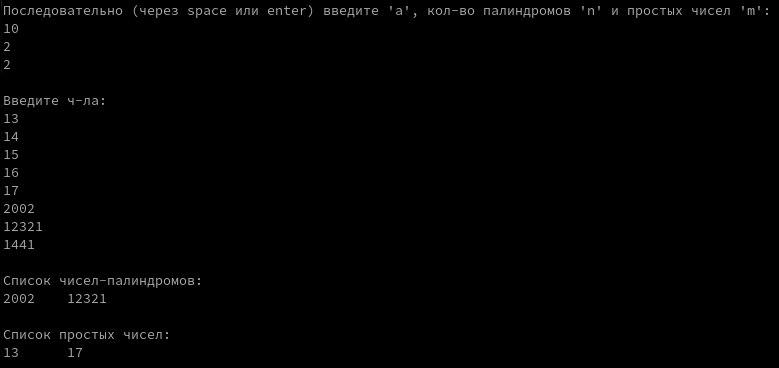
\includegraphics[width=1\textwidth]{first/report/1.png}
\end{document}
